\chapter{Kajian Pustaka}

\section{Pengenalan Emosi}
Emosi merupakan bagian dari komunikasi. Komunikasi berperan penting dalam interaksi sosial di beragam sistem sosial. Studi komunikasi merupakan studi multidisipliner yang melibatkan psikologi, sosiologi, antropologi dan linguistik \shortcite{mandal2014understanding}. \dots

\section{Penelitian Terkait}
\begin{figure}
    \centering
    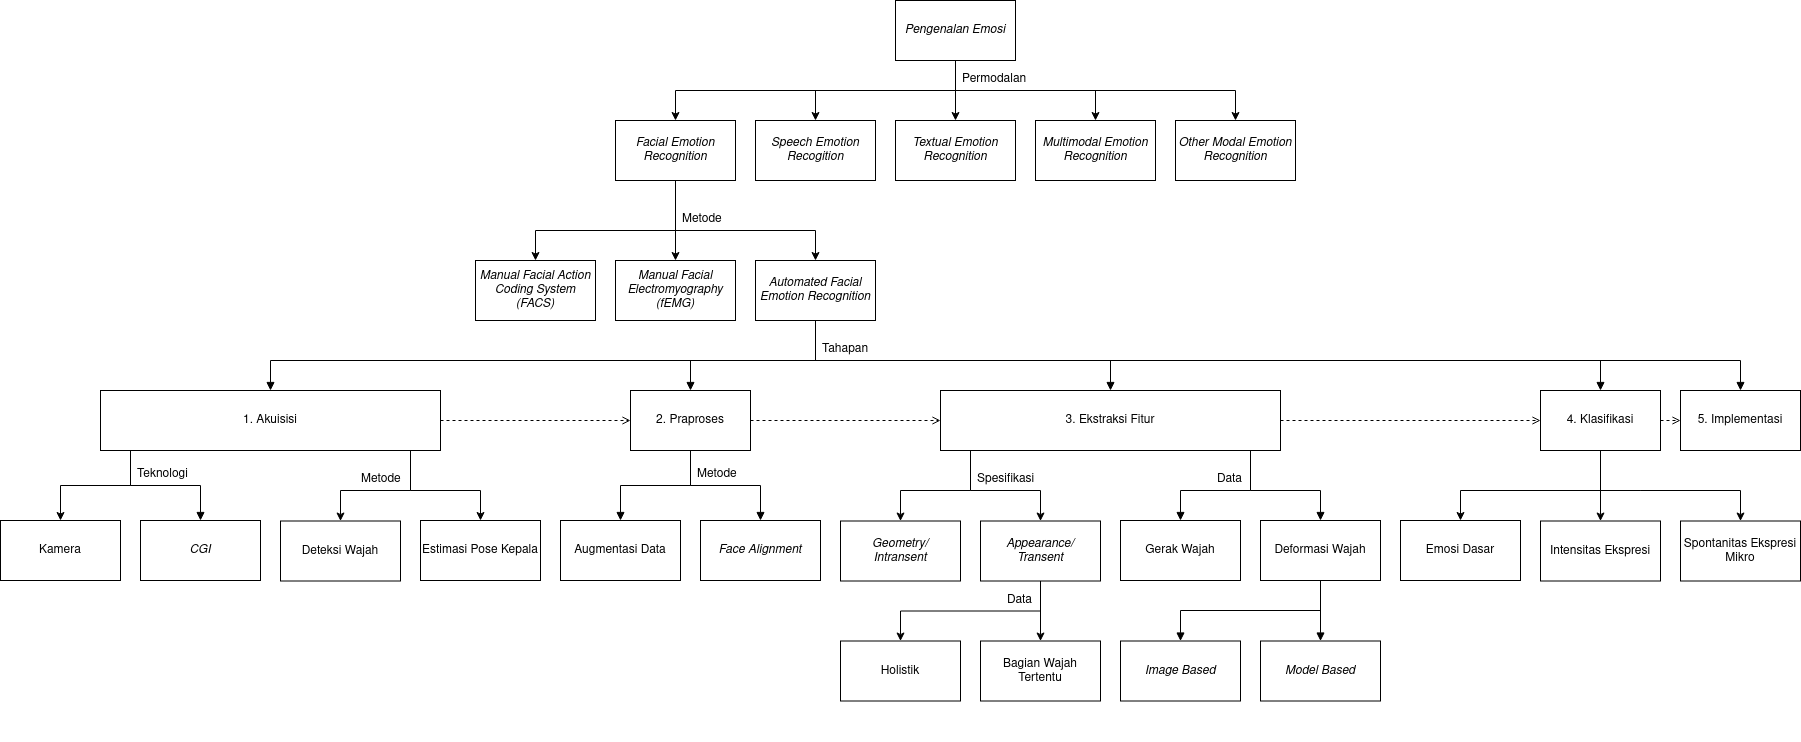
\includegraphics[width=14cm]{gambar/taksonomi_pengenalan_emosi.png}
    \caption[Taksonomi Pengenalan Emosi]{Taksonomi Pengenalan Emosi \protect\shortcite{sumathi2012automatic}}
    \label{fig:taksonomiemosi}
\end{figure}
Pengenalan emosi, terkait bidang ilmu komputer, memiliki domain penelitian yang sangat luas (Gambar \ref{fig:taksonomiemosi}). Berdasarkan jenis modal, pengenalan emosi dapat dilakukan baik melalui sinyal ucapan, tulisan, ekspresi wajah, sinyal digital ---seperti sinyal haptik dari \textit{drawing tablet} \shortcite{schrader2020linking}, sinyal aktifitas otak dari \textit{electroencephalogram} \shortcite{wagh2019electroencephalograph} dan sinyal tekanan dari \textit{keyboard} \shortcite{lv2008emotion}--- maupun kombinasi dari itu semua \shortcite{avots2019audiovisual,li2019fusion,mittal2019m3er}. \dots

\begin{wrapfigure}{r}{4.6cm}
    \centering
    \vspace{-12pt}
    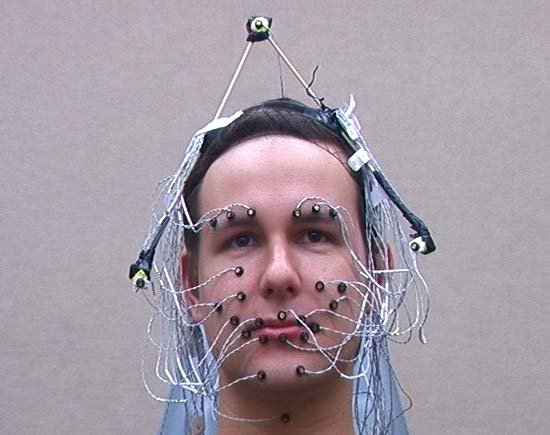
\includegraphics[width=4.5cm]{gambar/27_active_motion_capture_sensors.jpg}
    \caption[Contoh \emph{Facial Electromyography}]{Contoh \emph{Facial Electromyography} \protect\shortcite{gibert2010role}}
    \label{fig:contohfemg}
\end{wrapfigure}
Pengenalan emosi melalui ekspresi wajah menurut \shortciteA{wolf2015measuring} terbagi menjadi tiga metode, yaitu pelacakan aktivitas elektromiografi wajah, pengkodean aksi wajah dan rekognisi ekspresi wajah otomatis. Pelacakan aktivitas elektromiografi wajah atau \emph{facial electromyography} melibatkan penggunaan elektroda-elektroda yang dilekatkan pada permukaan wajah di titik-titik tertentu yang dianggap representatif (Gambar \ref{fig:contohfemg}). Sayangnya metode ini tidak dapat digunakan dalam situasi sosial sebab kompleksitas teknisnya. \dots

\begin{wrapfigure}[13]{l}{4.6cm}
    \centering
    \vspace{-12pt}
    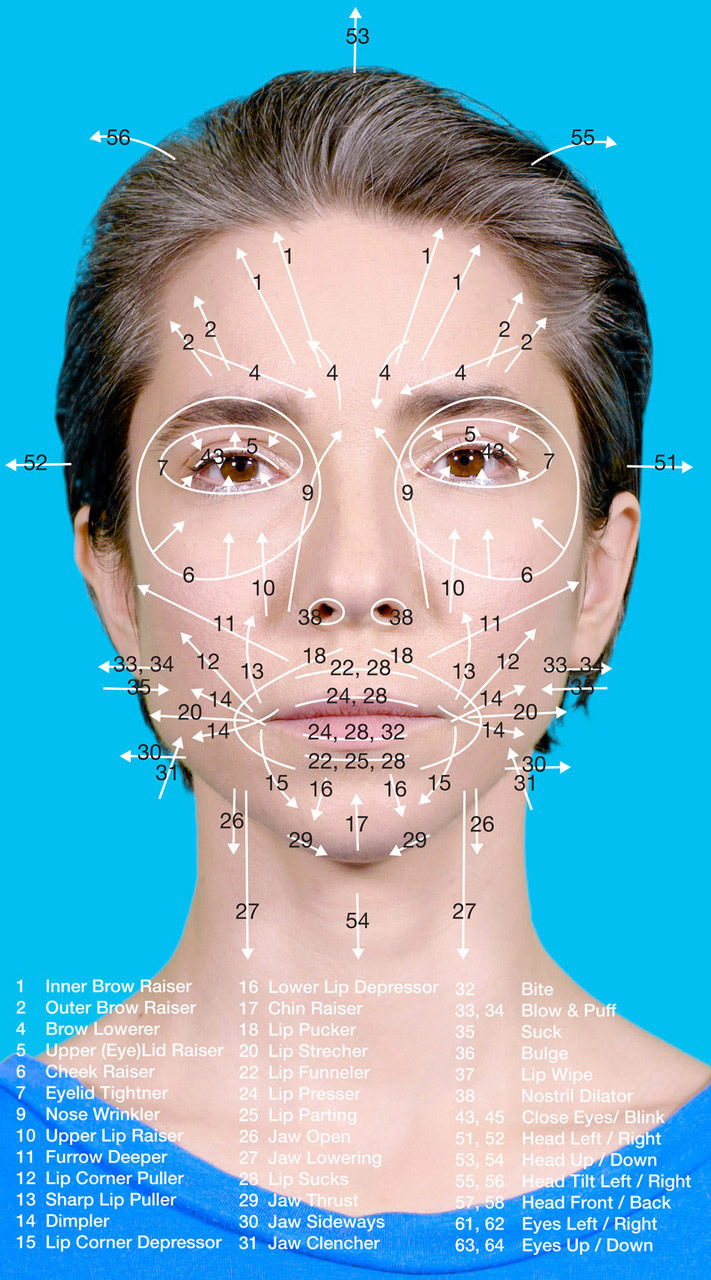
\includegraphics[width=4.425cm]{gambar/facs_coralie_vogelaar.jpg}
    \caption[Contoh \emph{Facial Action Units}]{Contoh \emph{Facial Action Units} (www.coralievogelaar.com)}
    \label{fig:contohfacs}
\end{wrapfigure}
Pengkodean aksi wajah atau \emph{facial action coding} \shortcite{ekman1997face} merupakan pengenalan emosi yang melibatkan analisis perubahan perilaku-perilaku otot-otot wajah yang kasat mata disebut sebagai unit aksi \emph{action units}. Unit-unit aksi ini didefinisikan secara manual, di antaranya adalah bagian kiri, kanan, luar dan dalam untuk tiap-tiap alis, mata, hidung, bibir dan mulut (Gambar \ref{fig:contohfacs}). Metode ini dapat meminimalkan bias oleh pengamat emosi. Namun proses analisis metode ini memerlukan bentukan emosi yang relatif kuat dan usaha manual yang banyak \shortcite{wolf2015measuring}. Dalam usaha meminimalkan waktu analisis pada perlakuan manual, pelacakan unit-unit aksi dikenali secara otomatis dengan pengukuran jarak relatif antar titik-titik wajah hasil deteksi tengara wajah atau \emph{facial landmarks} \shortcite{valstar2006fully}. \dots

\dots Tabel \ref{tab:penelitiansota} memberikan gambaran mengenai hasil penerapan berbagai usulan metode penelitian dalam pengenalan emosi otomatis melalui ekspresi wajah.

\begin{table}[ht]
    \caption{Penelitian Terkait}
    \label{tab:penelitiansota}
    \scriptsize
    \begin{tabular}{|C{1.4cm}|c|C{1.1cm}|C{2cm}|C{1.6cm}|C{1cm}|C{1cm}|c|}
        \hline
        \multicolumn{1}{|c|}{\multirow{2}{*}{Referensi}} & \multicolumn{1}{c|}{\multirow{2}{*}{Basis Data}} & \multicolumn{1}{C{1.1cm}|}{Tipe Jaringan} & \multicolumn{1}{C{2cm}|}{\multirow{2}{*}{Seleksi Data}} & \multicolumn{1}{c|}{\multirow{2}{*}{Praproses}} & \multicolumn{1}{C{1cm}|}{Ekstraksi Fitur} & \multicolumn{1}{c|}{\multirow{2}{*}{\textit{Classifier}}} & \multicolumn{1}{C{1cm}|}{Performa (\%)} \\
        \hline
        \shortciteNP{georgescu2019local} & \multirow{6}{*}{\centering FER-2013} & \multirow{2}{*}{\acrshort{cnn}, \emph{NE}} & \multirow{2}{*}{k-NN} & \multirow{4}{1.6cm}{\centering \emph{DA}} & \multirow{2}{1cm}{\centering \acrshort{cnn}s + BOVW} & \multirow{2}{*}{\centering SVM} & \multirow{2}{*}{\centering 75,42} \\
        \cline{1-1}\cline{3-4}\cline{6-8}
        \shortciteNP{agrawal2020using} &  & \multirow{4}{*}{\acrshort{cnn}} & \multirow{4}{2cm}{\centering 28.709 set \emph{training}, 3.589 set \emph{validation}, 3.589 set \emph{test}} &  & \multicolumn{2}{c|}{\multirow{2}{*}{CNN (17; 0,46M)$^\ast$}} & \multirow{2}{*}{65,23} \\
        \cline{1-1}\cline{5-8}
        \shortciteNP{engin2018face} &  &  &  & \multirow{2}{*}{\emph{PN}} & \multicolumn{2}{c|}{\multirow{2}{*}{VGG-face}} & \multirow{2}{*}{67,60} \\
        \hline
    \end{tabular}
    {\raggedright
    \emph{DA---Data Augmentation}; \emph{FA---Face Alignment}; \emph{FRS---Facial Region Segmentation}; \emph{IN---Illumination Normalization}; \emph{PN---Pose Normalization}; \emph{NE---Network Ensemble}; \emph{MN---Multitask Network}, \emph{CN---Cascaded Network} \\
    $^\ast$(Jumlah total lapisan bobot; jumlah total parameter \emph{training})} \\
\end{table}

\section{Filter Gabor}
Fungsi Gabor awalnya diperuntukkan dalam analisis sinyal saluran komunikasi, sebagai fungsi frekuensi terhadap waktu, guna mendapatkan esensi informasi \shortcite{gabor1946theory}. Fungsi ini diperluas menjadi fungsi \acrshort{2d} oleh \shortciteA{daugman1985uncertainty}, sebagai sebuah sinyal sinusoidal kompleks yang dimodulasi oleh fungsi Gaussian, yang dinyatakan \shortcite{grigorescu20062} dalam persamaan (\ref{equ:gabora}),
\begin{equation}
    g(x,y,\lambda,\theta,\psi,\sigma,\gamma) = \exp\left(-\frac{x'^2+\gamma^2y'^2}{2\sigma^2}\right) \cos\left(2\pi\frac{x'}{\lambda}+\psi\right)
    \label{equ:gabora}
\end{equation}
di mana,
\begin{description}[align=parleft,labelwidth=1cm]
    \item[$x'$] $= xcos(\theta) + ysin(\theta),$
    \item[$y'$] $= -xsin(\theta) + ycos(\theta),$
    \item[$\lambda$] $= \parbox[t]{11.35cm}{panjang gelombang faktor kosinus dari fungsi Gabor dengan nilai bilangan riil yang valid 2--256 piksel,}$
    \item[\dots] $\dots$
\end{description}
